% Created 2024-06-14 Fri 10:33
% Intended LaTeX compiler: pdflatex
\documentclass[11pt]{article}
\usepackage[utf8]{inputenc}
\usepackage[T1]{fontenc}
\usepackage{graphicx}
\usepackage{longtable}
\usepackage{wrapfig}
\usepackage{rotating}
\usepackage[normalem]{ulem}
\usepackage{amsmath}
\usepackage{amssymb}
\usepackage{capt-of}
\usepackage{hyperref}
\usepackage{minted}
\usepackage{xcolor}
\usepackage{hyperref}
\usepackage{tocloft}
\usepackage[margin=1.8cm]{geometry}
\usepackage{fancyheadings}
\usepackage{minted}
\usepackage[utf8]{inputenc}
\usepackage{amsmath}
\usepackage{amsfonts}
\usepackage{amssymb}
\usepackage{titlesec}
\usemintedstyle{manni}
\usepackage{enumitem}
\usepackage{pdfpages}
\setlength{\parindent}{0cm}
\usepackage{parskip}
\usemintedstyle{friendly}
\usepackage{graphicx}
\usepackage{listings}
\usepackage{float}
\usepackage{tabularx}
\usepackage{color}
\usepackage{tabularray}
\restylefloat{table}
\usemintedstyle{dracula}
\usepackage[table]{xcolor}
\usepackage{setspace}
\usepackage[none]{hyphenat}
\usepackage{xcolor}
\usepackage{pagecolor}
\definecolor{solarizedBase03}{RGB}{0, 43, 54}
\definecolor{solarizedBase02}{RGB}{7, 54, 66}
\definecolor{solarizedBase01}{RGB}{88, 110, 117}
\definecolor{solarizedBase00}{RGB}{101, 123, 131}
\definecolor{solarizedBase0}{RGB}{131, 148, 150}
\definecolor{solarizedBase1}{RGB}{147, 161, 161}
\definecolor{solarizedBase2}{RGB}{238, 232, 213}
\definecolor{solarizedBase3}{RGB}{253, 246, 227}
\definecolor{solarizedYellow}{RGB}{181, 137, 0}
\definecolor{solarizedOrange}{RGB}{203, 75, 22}
\definecolor{solarizedRed}{RGB}{220, 50, 47}
\definecolor{solarizedMagenta}{RGB}{211, 54, 130}
\definecolor{solarizedViolet}{RGB}{108, 113, 196}
\definecolor{solarizedBlue}{RGB}{38, 139, 210}
\definecolor{solarizedCyan}{RGB}{42, 161, 152}
\definecolor{solarizedGreen}{RGB}{133, 153, 0}
\pagecolor{solarizedBase3}
\color{solarizedBase00}
\hypersetup{
colorlinks=true,
linkcolor=solarizedViolet,
filecolor=solarizedMagenta,
urlcolor=solarizedBlue,
citecolor=solarizedGreen,
}
\titleformat{\section}
{\color{solarizedBlue}\normalfont\Large\bfseries}
{\color{solarizedBlue}\thesection}{1em}{}
\titleformat{\subsection}
{\color{solarizedGreen}\normalfont\large\bfseries}
{\color{solarizedGreen}\thesubsection}{1em}{}
\titleformat{\subsubsection}
{\color{solarizedYellow}\normalfont\normalsize\bfseries}
{\color{solarizedYellow}\thesubsubsection}{1em}{}
\usepackage{colortbl}
\usepackage{booktabs}
\definecolor{draculaBackground}{HTML}{282a36}
\definecolor{draculaForeground}{HTML}{f8f8f2}
\definecolor{draculaSelection}{HTML}{44475a}
\definecolor{draculaComment}{HTML}{6272a4}
\definecolor{draculaCyan}{HTML}{8be9fd}
\definecolor{draculaGreen}{HTML}{50fa7b}
\definecolor{draculaOrange}{HTML}{ffb86c}
\definecolor{draculaPink}{HTML}{ff79c6}
\definecolor{draculaPurple}{HTML}{bd93f9}
\definecolor{draculaRed}{HTML}{ff5555}
\definecolor{draculaYellow}{HTML}{f1fa8c}
\author{Rob Alicea}
\date{\today}
\title{P.S. 192 The Parent Newsletter- Edition- June-2024}
\hypersetup{
 pdfauthor={Rob Alicea},
 pdftitle={P.S. 192 The Parent Newsletter- Edition- June-2024},
 pdfkeywords={},
 pdfsubject={},
 pdfcreator={Emacs 29.3 (Org mode 9.6.24)}, 
 pdflang={English}}
\begin{document}

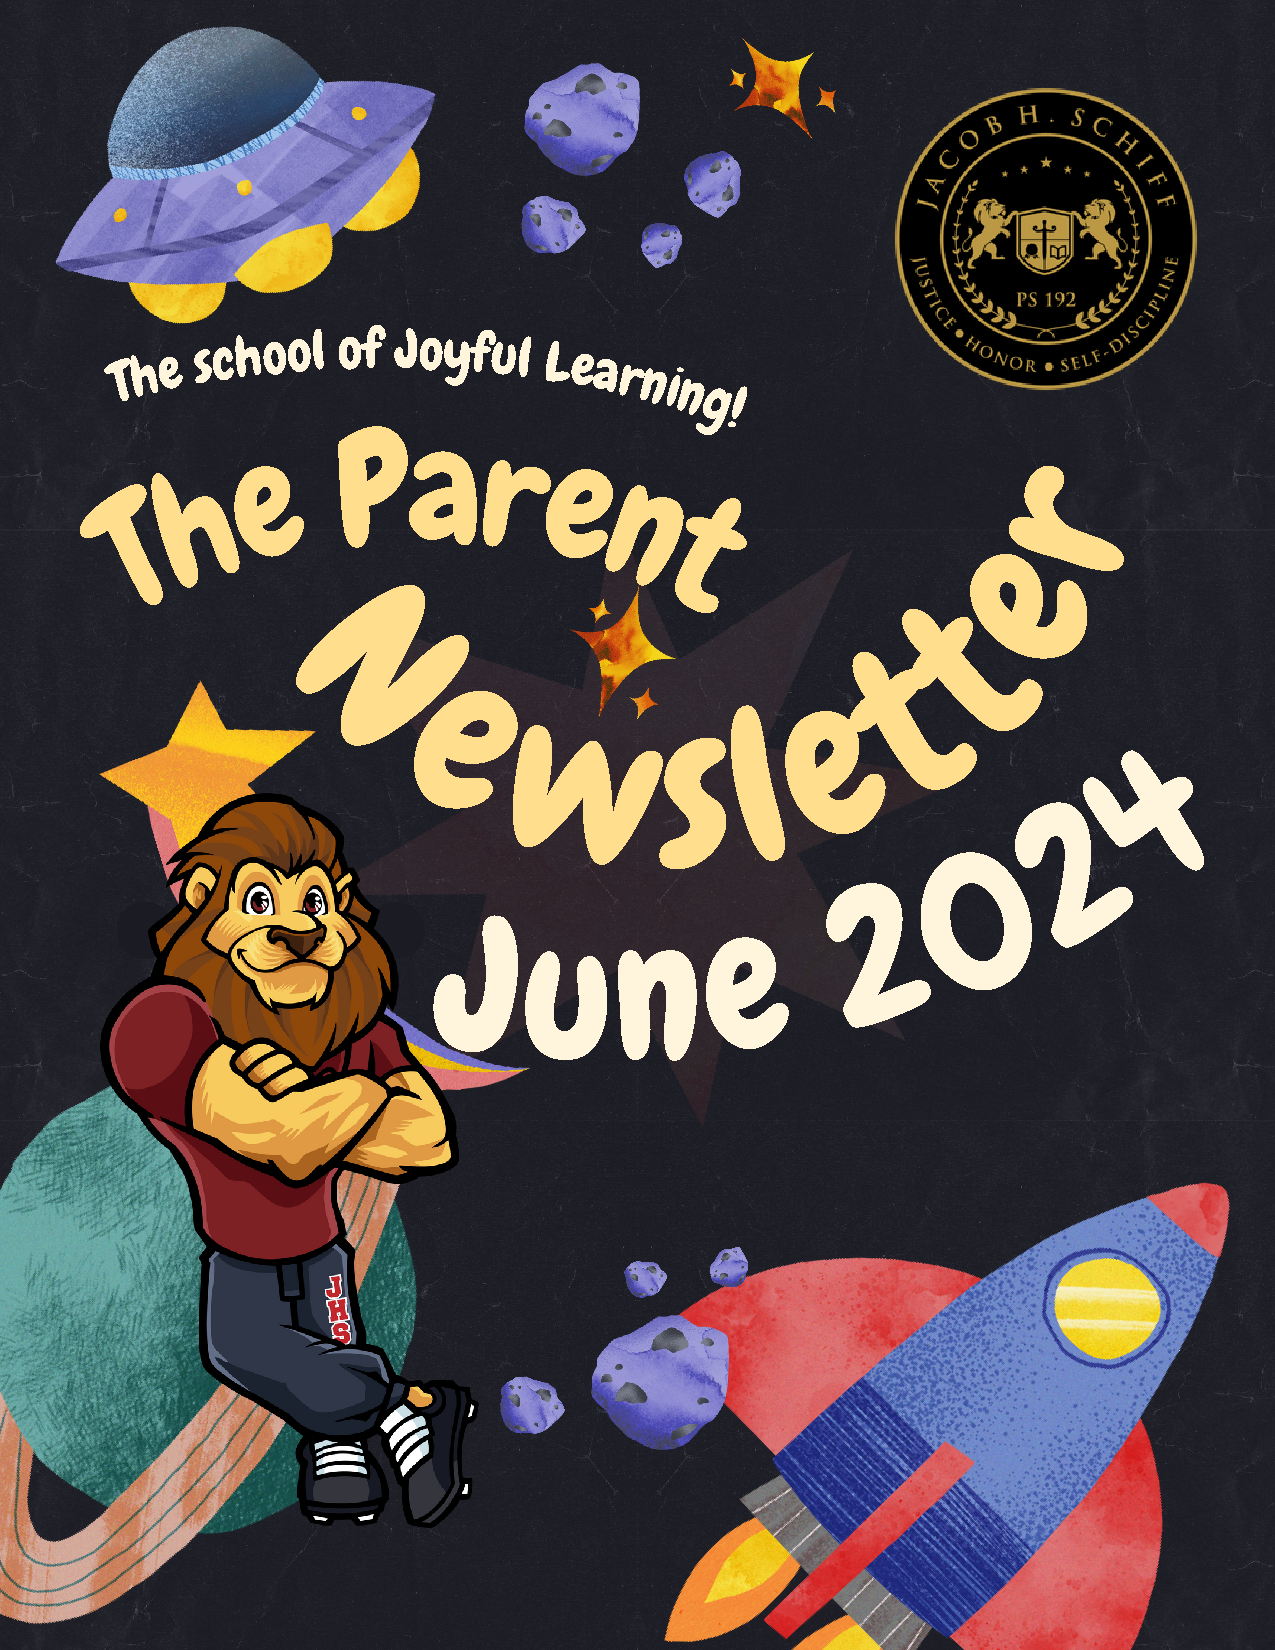
\includepdf[pages=1,fitpaper]{pdf.pdf}

\pagenumbering{\fancyhf{}}
\pagestyle{headings}
\pagenumbering{arabic}

\fancyhead[R]{\thepage}

\fancyfoot[C]{Visit www.ps192.org | The School of Joyful Learning!}
\pagestyle{fancy}
\renewcommand{\footrulewidth}{1px}

\definecolor{dkgreen}{rgb}{0,0.6,0}
\definecolor{gray}{rgb}{0.5,0.5,0.5}
\definecolor{mauve}{rgb}{0.58,0,0.82}

\clearpage
\clearpage \tableofcontents \clearpage


\section{Principal Message}
\label{sec:orgc464f31}

\textbf{Subject: Welcome to June, 2024 at PS 192: The School of Joyful Learning!}

Greetings Parents and Guardians,

As we approach the end of this school year, I am filled with immense pride for the achievements we have made together at P.S. 192 and am equally excited about the plans we have for the upcoming school year.

I extend my heartfelt gratitude to all parents who have contributed to our school events throughout the year. Your dedication in organizing and participating in our activities and your steadfast attendance at our parent workshops have been invaluable. Your unwavering support has made a significant impact on our school community.

Please note that Wednesday, June 26, 2024, will be our Graduation Day and the final day of school. On this day, your children will receive their report cards.

In closing, I would like to wish our fifth-grade students the very best as they transition to Middle School. I will miss each of you and your families and hope you carry with you cherished memories of your time at P.S. 192.

I wish everyone a delightful and restful summer and look forward to collaborating with many of you in the upcoming year.

Warm regards,


\includegraphics[width=100px]{/var/home/rob/Documents/latex_documents/Newsletters/June_solirize_light/hil_signature.png}

\textbf{Hilduara Abreu}

Principal
\clearpage

\section{Inspiration Corner}
\label{sec:orgbcc62a4}
\subsection{P.S. 192 Parents}
\label{sec:org06381f7}
You always need to remember to bring your photo I.D when you come to your child’s school.

\begin{figure}[htbp]
\centering

\includegraphics[width=1\textwidth]{/var/home/rob/Documents/latex_documents/Newsletters/June_solirize_light/lion_banner.png}
\caption{Infinite Potential is the guiding star of our school, illuminating a path where students are emboldened to dream without boundaries and pursue a voyage of continuous learning and self-improvement. It is here, within the nurturing halls of PS192, that we ignite the spark of curiosity and fan the flames of possibility, forging a future replete with endless opportunities for each and every child.}
\end{figure}
\subsection{P.S. 192 Quote}
\label{sec:orgcc4d13d}
``True happiness lies not in the destination, but in the journey we take with our children, nurturing their growth, celebrating their successes, and guiding them with love and patience. As parents and guardians, your support and dedication light up the path to a brighter future for our students at P.S. 192.''
\subsection{Graduation}
\label{sec:org9daed1d}
June 26, 2024
\begin{itemize}
\item \textbf{3K \& PRE-K}- 8:30 AM
\item \textbf{Kindergarten}- 10:00 AM
\item \textbf{5th Grade}- 12:30 PM
\end{itemize}
\subsection{Last Day of School}
\label{sec:orga049984}
June 26th, 2024

\textbf{Have a wonderful Summer!}
\clearpage
\section{Special Days and News of the Month}
\label{sec:orge89e75c}
\begin{center}
\definecolor{JordyBlue}{rgb}{0.6,0.756,0.945}
\definecolor{Carnation}{rgb}{0.964,0.38,0.317}
\begin{table}[h!]
\centering
\caption{For comprehensive and up-to-date information regarding P.S. 192, we invite you to visit our official website at www.ps192.org. The site is regularly updated with the latest school events and pertinent details. Additionally, our news (www.ps192.org/apps/news/) section offers exclusive insights into the happenings at our school. We encourage you to explore the wealth of resources available there.}
\begin{tblr}{
  width = \linewidth,
  colspec = {Q[133]Q[810]},
  row{odd} = {Carnation},
  row{1} = {JordyBlue},
  hlines,
  vlines,
}
\textbf{Date}       & \textbf{Event}                                                                    \\
\textbf{06/06/2024} & \textbf{Chancellor’s Conference Day- Staff Development (school Closed)}           \\
\textbf{06/07/2024} & \textbf{Clerical Day- Staff Development (School Closed) AM}                       \\
\textbf{06/07/2024} & \textbf{SLT- 2:30 - 5:30 PM}                                                      \\
\textbf{06/12/2024} & \textbf{Senior Trip}                                                              \\
\textbf{06/14/2024} & \textbf{Travel The World Day}                                                     \\
\textbf{06/17/2024} & \textbf{Eid al-Adha- No School}                                                   \\
\textbf{06/18/2024} & \textbf{School Resumes}                                                           \\
\textbf{06/18/2024} & \textbf{P.A. Election 8:00 AM}                                                    \\
\textbf{06/18/2024} & \textbf{Coffee with The Principal- 8:15 AM}                                       \\
\textbf{06/19/2024} & \textbf{Juneteenth Day- schools closed}                                           \\
\textbf{06/21/2024} & \textbf{Field Day}                                                                \\
\textbf{06/24/2024} & \textbf{5th Grade Prom- 11:00 AM – 2:00 P}                                        \\
\textbf{06/25/2024} & \textbf{Awards Ceremony- Grades 3K-5th 1:00 – 2:00 PM}                            \\
\textbf{06/26/2024} & \textbf{Graduation 3K - PRE-K 8:30 AM, Kindergarten 10:00 AM, 5th Grade 12:30 PM} \\
\textbf{06/26/2024} & \textbf{Last Day For All Students}
\end{tblr}
\end{table}
\end{center}

\section{What's Next}
\label{sec:orgffdb87e}
\subsection{Looking Forward to Next Month}
\label{sec:orgb5708bd}
\begin{itemize}
\item \texttt{Independence Day} – July 4, 2024 (school is closed)
\item \texttt{First day of Summer School} – July 2nd, 2024.
\item \texttt{Last day of Summer School} – August 16th, 2024.
\end{itemize}

\textbf{\Larger Have a wonderful vacation! We will see you on September 5, 2024.}
\begin{figure}[htbp]
\centering
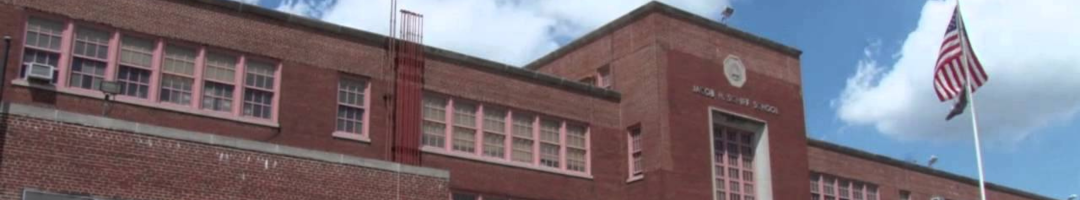
\includegraphics[width=1\textwidth]{/var/home/rob/Documents/latex_documents/Newsletters/June_solirize_light/school_banner.png}
\caption{School Motto ``Good, better, best. Never let it rest until your good is better, and your better is best.'' St. Jerome}
\end{figure}
\section{Reminder}
\label{sec:orgeed60c0}
\begin{enumerate}
\item School Uniform Reminder: Please ensure your child comes to school dressed in their uniform daily, as it is an important part of our school's tradition and identity.
\item ID. To ensure the safety of children, and as per DOE regulation, you always need to bring your photo I.D when you come to your child’s school.
\item We highly recommend taking the time each week to touch base with your child's teachers. Whether through email, in-person meetings, ClassDojo, or virtual conferences, staying connected can greatly enhance your child's educational experience.
\item Library Mornings Program- We would like to inform all Parents and Guardians that the library is open for your use with your children from Monday to Friday, 7:00 to 7:50 am. This is a wonderful opportunity for you to borrow books, work on computers, and practice reading.
\item Lost Items - Please note that if your child misplaces any belongings, you are encouraged to visit the lost and found area. Items that remain unclaimed by the end of each month will be thoughtfully donated to the Salvation Army.
\end{enumerate}
\end{document}
